% =====================================================================
% Lab 04 --- Item 2.5: polares de arrasto
% Incluido por main.tex. Tabelas em tex_q5/ e figuras em
% resultados_q5/ (mesmo nivel que este arquivo e o main.tex).
% Codigos em polares/.
% =====================================================================
% gerado por q5_polares.py
\newcommand{\poAlphaAftLivre}{0.04}
\newcommand{\poAlphaAftTrim}{0.04}
\newcommand{\poAlphaFwdLivre}{0.18}
\newcommand{\poAlphaFwdTrim}{0.18}
\newcommand{\poAlt}{10668}
\newcommand{\poCDAftLivre}{0.02023}
\newcommand{\poCDAftTrim}{0.02023}
\newcommand{\poCDFwdLivre}{0.02081}
\newcommand{\poCDFwdTrim}{0.02081}
\newcommand{\poCDaFit}{0.18763}
\newcommand{\poCDaaFit}{1.48578}
\newcommand{\poCDdt}{0.02183}
\newcommand{\poCDzeroDT}{0.01328}
\newcommand{\poCDzeroFit}{0.02010}
\newcommand{\poCLmaxAftLivre}{0.877}
\newcommand{\poCLmaxAftTrim}{0.882}
\newcommand{\poCLmaxFwdLivre}{0.864}
\newcommand{\poCLmaxFwdTrim}{0.854}
\newcommand{\poCLmin}{-0.5}
\newcommand{\poCLproj}{0.4702}
\newcommand{\poDeAftLivre}{+0.00}
\newcommand{\poDeAftTrim}{+0.00}
\newcommand{\poDeFwdLivre}{+0.00}
\newcommand{\poDeFwdTrim}{-0.00}
\newcommand{\poDifAbsAftLivre}{7.3}
\newcommand{\poDifAbsAftTrim}{7.3}
\newcommand{\poDifAbsFwdLivre}{4.7}
\newcommand{\poDifAbsFwdTrim}{4.7}
\newcommand{\poDifAftLivre}{-7.3}
\newcommand{\poDifAftTrim}{-7.3}
\newcommand{\poDifFwdLivre}{-4.7}
\newcommand{\poDifFwdTrim}{-4.7}
\newcommand{\poEffAftLivre}{23.2}
\newcommand{\poEffAftTrim}{23.2}
\newcommand{\poEffDT}{21.5}
\newcommand{\poEffFwdLivre}{22.6}
\newcommand{\poEffFwdTrim}{22.6}
\newcommand{\poItAft}{-1.959}
\newcommand{\poItFwd}{-3.429}
\newcommand{\poIw}{4.5}
\newcommand{\poMach}{0.85}
\newcommand{\poRdois}{0.99999}


\section{Item 5 --- Polares de arrasto}
\label{sec:polares}

\subsection{Montagem das curvas}

As quatro polares pedidas pelo enunciado foram levantadas no Mach e na altitude
do ponto de projeto ($M = \poMach$, $h = \poAlt$~m), com a incidência de
empenagem do item~3 e todas as superfícies de alta sustentação neutras:

\begin{enumerate}[label=(\alph*)]
  \item CG dianteiro sem deflexões de superfície de controle
  ($\delta_e$ travado em zero);
  \item CG traseiro sem deflexões de superfície de controle;
  \item CG dianteiro com arfagem compensada ($C_M = 0$);
  \item CG traseiro com arfagem compensada ($C_M = 0$).
\end{enumerate}

Em vez de varrer $\alpha$ e depois recortar, usou-se diretamente a restrição de
$C_L$ do AVL (comando \code{a c}), o que faz cada curva nascer e morrer
exatamente onde o enunciado pede: de $C_L = \poCLmin$ até o $C_{L\,max}$
calculado pelo método da seção crítica no item~4, que é específico de cada
caso (Tab.~\ref{tab:secao-critica}). Nos casos (a) e (b) o profundor é travado
em zero (\code{d4 d4 0}); nos casos (c) e (d) entra a restrição de trimagem
(\code{d4 pm 0}). O ponto de projeto foi incluído na grade de $C_L$ para ser
lido sem interpolação.

\subsection{Resultados}

A Fig.~\ref{fig:polar} traz as quatro polares em um único gráfico, junto com a
polar do \code{designTool} na mesma condição, e a Fig.~\ref{fig:polar-zoom}
amplia a vizinhança do ponto de projeto, onde as curvas se distinguem.

\begin{figure}[H]
\centering
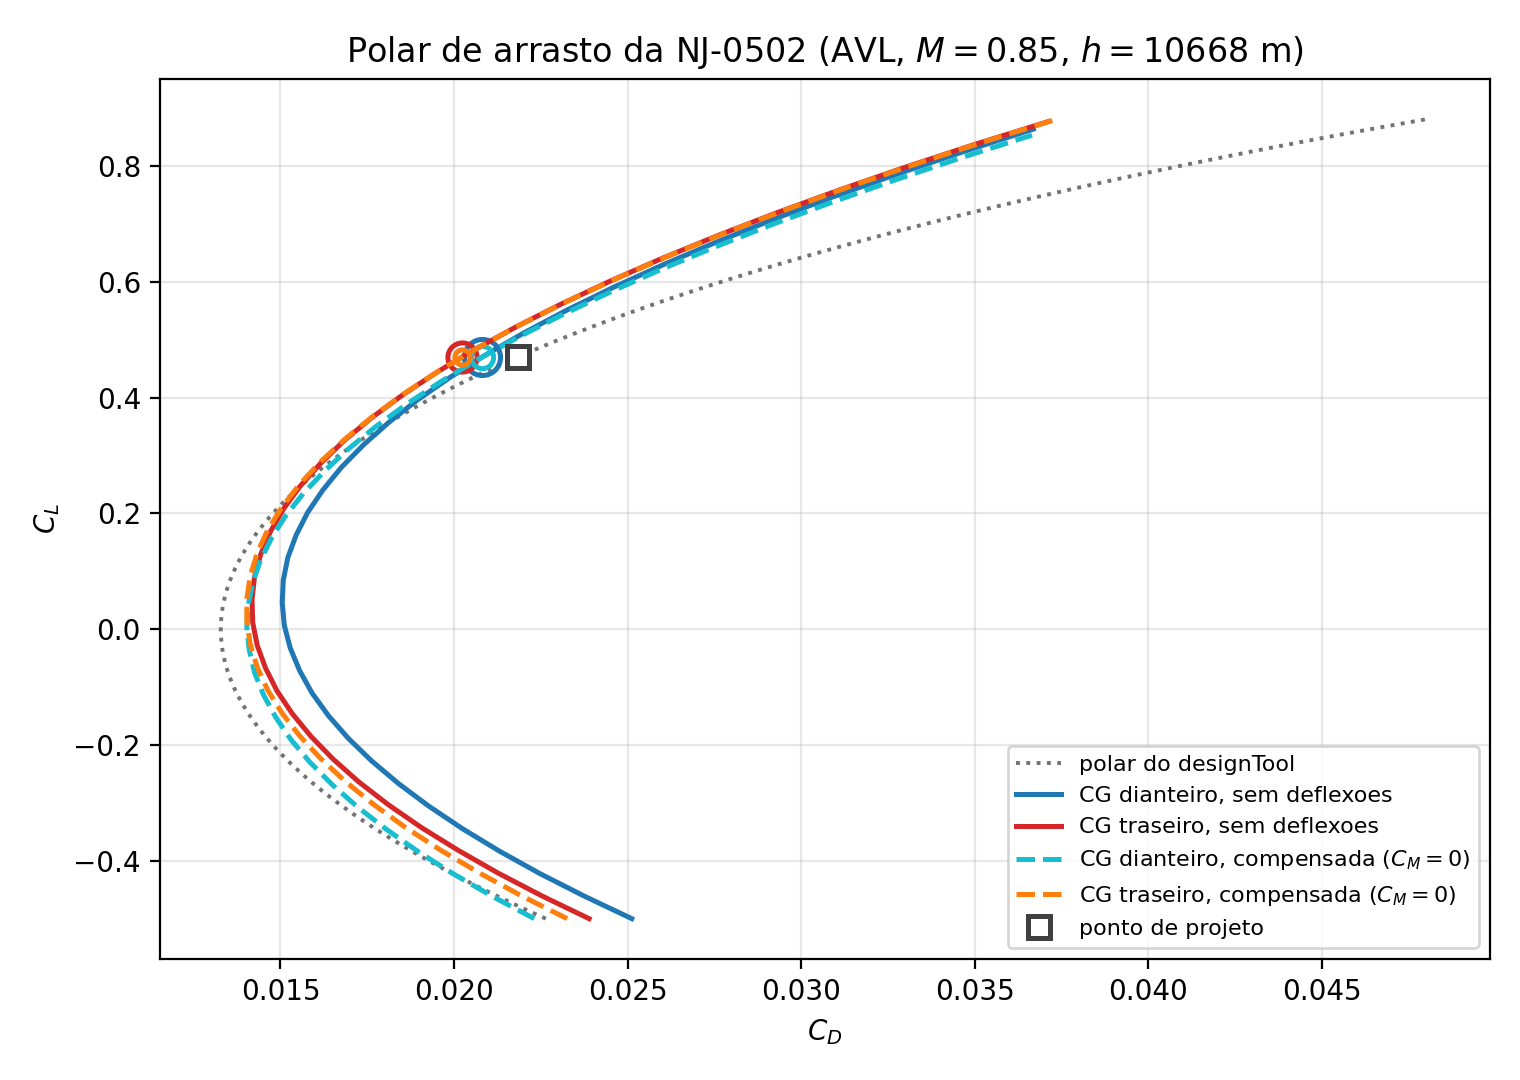
\includegraphics[width=0.74\textwidth]{resultados_q5/polar_CD_CL.png}
\caption{Polares de arrasto da NJ-0502 no ponto de projeto
($M=\poMach$, $h=\poAlt$~m). Cada curva termina no $C_{L\,max}$ do item~4.
Os círculos marcam o ponto de projeto ($C_L = \poCLproj$) e o quadrado, o ponto
de projeto segundo a polar do \code{designTool}.}
\label{fig:polar}
\end{figure}

\begin{figure}[H]
\centering
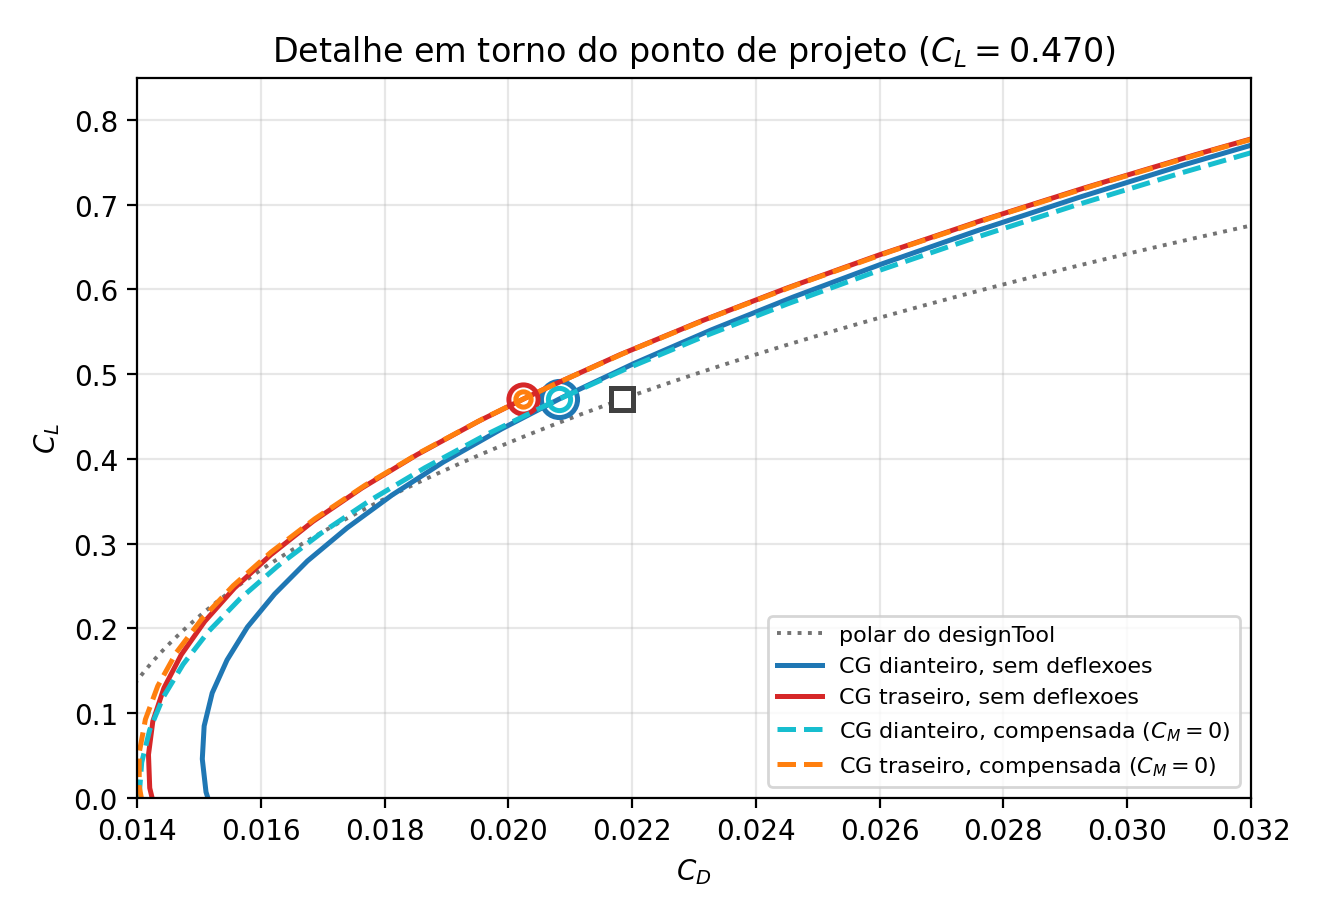
\includegraphics[width=0.7\textwidth]{resultados_q5/polar_CD_CL_zoom.png}
\caption{Detalhe das polares em torno do ponto de projeto.}
\label{fig:polar-zoom}
\end{figure}

\begin{table}[H]
\centering
\caption{$C_D$ no $C_L$ do ponto de projeto ($C_L = \poCLproj$) para as quatro
configurações, comparado com o valor da polar do \code{designTool}.}
\label{tab:CD-ponto}
\begin{tabular}{lccccc}
\toprule
Configuracao & $\alpha$ [$^\circ$] & $\delta_e$ [$^\circ$] & $C_D$ (AVL) & $C_D$ (designTool) & dif. \\
\midrule
CG dianteiro, sem deflexoes & 0.18 & $+0.00$ & 0.02081 & 0.02183 & $-4.7$\% \\
CG traseiro, sem deflexoes & 0.04 & $+0.00$ & 0.02023 & 0.02183 & $-7.3$\% \\
CG dianteiro, compensada ($C_M=0$) & 0.18 & $+0.00$ & 0.02081 & 0.02183 & $-4.7$\% \\
CG traseiro, compensada ($C_M=0$) & 0.04 & $+0.00$ & 0.02023 & 0.02183 & $-7.3$\% \\
\bottomrule
\end{tabular}

\end{table}

\subsection{Discussão}

\paragraph{Efeito do CG e da trimagem no ponto de projeto.}
As quatro configurações praticamente coincidem no ponto de projeto:
$C_D = \poCDFwdLivre$ no CG dianteiro e $\poCDAftLivre$ no CG traseiro, com
diferença desprezível entre as versões trimada e não trimada
($\delta_e = \poDeFwdTrim^\circ$ e $\poDeAftTrim^\circ$). Isso não é
coincidência: é a verificação numérica do item~3. O $i_t$ de cada arquivo foi
escolhido justamente para anular o profundor nesse $C_L$, de modo que trimar ou
não trimar dá o mesmo resultado \emph{ali}. A separação entre as curvas cheias e
tracejadas na Fig.~\ref{fig:polar} cresce à medida que se afasta do ponto de
projeto, e é onde aparece o arrasto de trimagem.

A pequena vantagem do CG traseiro ($\poDifAftLivre$\% contra
$\poDifFwdLivre$\% em relação ao \code{designTool}) tem a mesma origem: com o CG
mais atrás, o $i_t$ necessário é menos negativo ($\poItAft^\circ$ contra
$\poItFwd^\circ$), a carga descendente na empenagem é menor e a asa precisa
gerar menos sustentação --- logo menos arrasto induzido. É o argumento clássico
a favor de voar com o CG o mais atrás que a margem estática permitir.

\paragraph{Comparação com a polar do \code{designTool}.}
O AVL fica \poDifAbsAftLivre\% \emph{abaixo} do \code{designTool}
($C_D = \poCDdt$) no ponto de projeto, o que corresponde a uma eficiência
$C_L/C_D$ de \poEffAftLivre{} contra \poEffDT{}. A diferença tem duas origens
identificáveis:

\begin{itemize}
  \item o \textbf{arrasto parasita é o mesmo por construção}: o campo
  \code{\# CDp} dos arquivos \code{.avl} recebeu o próprio $C_{D0}$ de cruzeiro
  do \code{designTool} ($\poCDzeroDT$), e o AVL o devolve intacto na linha
  \code{CDvis}. Não há divergência a explicar aqui;
  \item a diferença está toda no \textbf{arrasto induzido e de onda}. O AVL
  resolve a distribuição de sustentação da asa real e obtém um fator de
  Oswald próprio, enquanto o \code{designTool} usa a correlação
  $C_{D} = C_{D0} + K C_L^{2}$ com um $K$ que já embute uma parcela de arrasto de
  onda em $M = \poMach$. Como o AVL é um método potencial linear, ele
  \emph{não modela arrasto de onda nenhum} --- e é exatamente essa parcela que
  falta.
\end{itemize}

A conclusão prática é que as duas estimativas não são substituíveis: o AVL é
melhor para o arrasto induzido e para capturar o efeito de CG e de trimagem,
mas subestima o arrasto total em cruzeiro transônico. Para o desempenho da
aeronave em $M = \poMach$ o valor do \code{designTool} continua sendo o
mais adequado; a contribuição do AVL aqui é mostrar que a parcela induzida está
bem estimada e quantificar o custo de trimagem fora do ponto de projeto.

\paragraph{Ajuste quadrático para a Seção~3 (Tab.~7 do enunciado).}
A polar não trimada de CG traseiro (caso 5.b) foi ajustada por
$C_D = C_{D0} + C_{D\alpha}\,\alpha + C_{D\alpha^{2}}\,\alpha^{2}$, com $\alpha$
em radianos, na faixa de $C_L$ de $-0{,}1$ ao $C_{L\,max}$
(Fig.~\ref{fig:ajuste} e Tab.~\ref{tab:ajuste}). O ajuste é excelente
($R^{2} = \poRdois$), como era de esperar de uma polar essencialmente
parabólica.

\textbf{Atenção: o $C_{D0}$ deste ajuste não é o arrasto parasita.} O termo
constante vale $\poCDzeroFit$, bem acima do $C_{D0}$ de $\poCDzeroDT$ que foi
\emph{dado} ao AVL no campo \code{\# CDp}. Não há contradição --- são grandezas
diferentes. Como a asa está a $i_w = \poIw^\circ$ (item~3), $\alpha = 0$ é a
atitude de \emph{fuselagem nivelada}, que é praticamente o próprio ponto de
projeto: ali o avião já gera $C_L \approx \poCLproj$ e, com ele, todo o arrasto
induzido correspondente. Por isso $\poCDzeroFit \approx \poCDAftLivre$, o $C_D$
do ponto de projeto.

Essa é exatamente a forma que o modelo de MVO espera, porque lá o $\alpha$
também é medido a partir da linha de referência da fuselagem. O preço é que o
termo linear deixa de ser desprezível: $C_{D\alpha} = \poCDaFit$/rad, contra um
valor quase nulo que se obteria se $\alpha$ fosse contado da sustentação nula.
Ao transcrever a Tab.~\ref{tab:ajuste} para a Seção~3, portanto, é preciso usar
os três coeficientes juntos --- o $C_{D0}$ isolado não tem o significado de
arrasto parasita.

\begin{figure}[H]
\centering
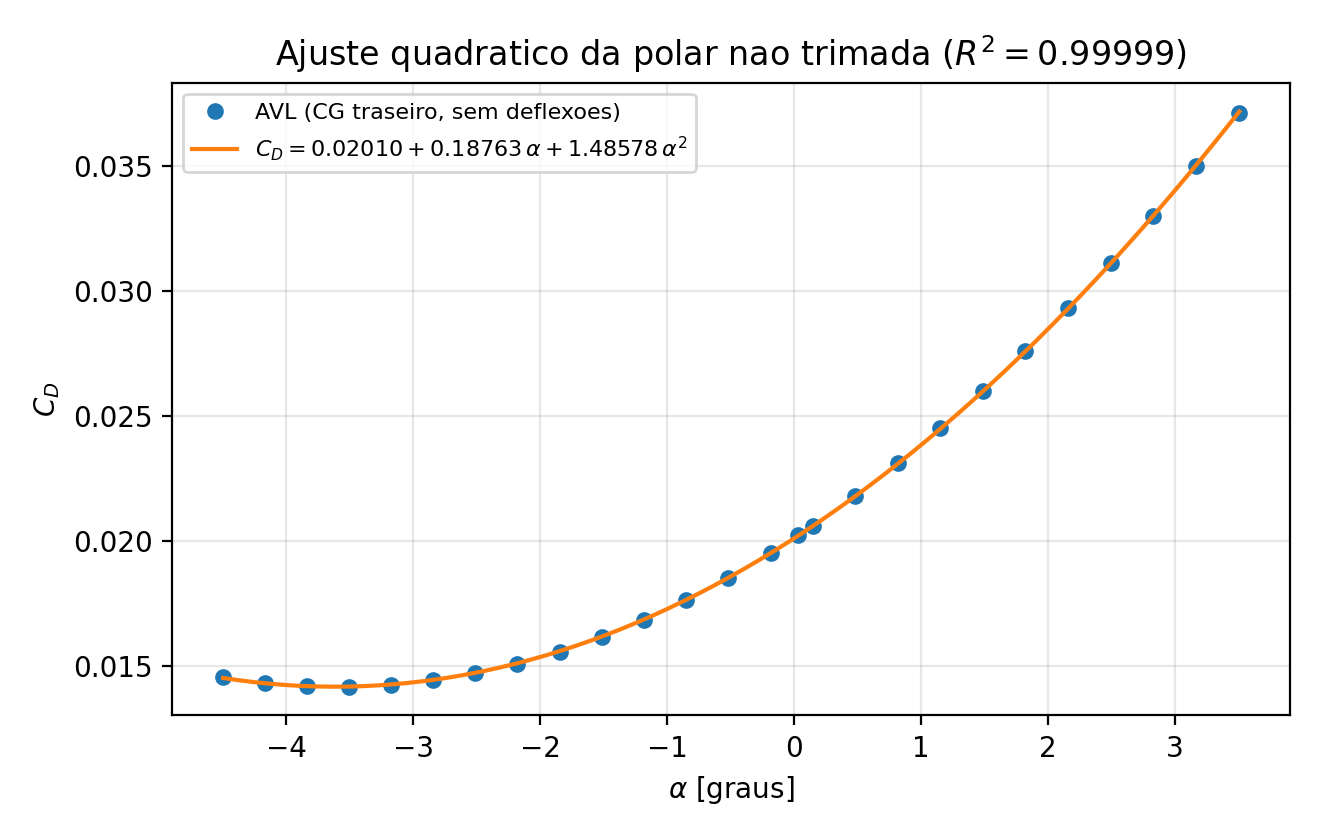
\includegraphics[width=0.68\textwidth]{resultados_q5/ajuste_CD_alpha.png}
\caption{Ajuste quadrático da polar não trimada de CG traseiro, usado para
preencher a Tab.~7 do enunciado.}
\label{fig:ajuste}
\end{figure}

\begin{table}[H]
\centering
\caption{Ajuste quadrático da polar de arrasto não trimada (exercício 5.b).}
\label{tab:ajuste}
\begin{tabular}{llr}
\toprule
Parametro & Explicacao & Valor \\
\midrule
$C_{D0}$ & termo constante ($\alpha$ da fuselagem; nao e o arrasto parasita) & 0.02010 \\
$C_{D\alpha}$ & termo linear [1/rad] & 0.18763 \\
$C_{D\alpha^2}$ & termo quadratico [1/rad$^2$] & 1.48578 \\
\bottomrule
\end{tabular}

\end{table}

\paragraph{Faixa de validade das curvas.}
Como cada polar termina no $C_{L\,max}$ de baixa velocidade do item~4, os
trechos de $C_L$ alto das curvas da Fig.~\ref{fig:polar} são formalmente
inconsistentes: eles estão traçados em $M = \poMach$, condição em que a
aeronave nunca chegaria a $C_L = \poCLmaxAftLivre$ sem antes entrar em estol de
onda (\emph{shock stall}), bem antes do estol de bordo de ataque calculado no
item~4. O corte foi mantido porque é o que o enunciado pede, mas na prática
apenas a região $0{,}3 \lesssim C_L \lesssim 0{,}6$ dessas curvas representa
condições de voo realizáveis em cruzeiro. Os arquivos
\code{resultados\_q5/polar\_*.csv} guardam $\alpha$, $\delta_e$ e $C_M$ de
cada ponto, o que permite refazer as curvas em outra condição sem rodar o AVL
de novo.
